\section{Overview}
\label{overview}

\noindent
Each Apache Spark job typically consists of multiple execution stages where each stage implements certain operations and is executed sequentially. Moreover, to facilitate parallel processing, input data set is partitioned into multiple sets and are distributed over multiple worker nodes. Within each worker node, multiple batches of tasks are launched to process the corresponding partition of the input data. The number of tasks within each node is determined based on the size of the input data and configuration settings of the program. For example, if the input data size of the PageRank job is 2.5 GB, the total number of input blocks will be 40 for a default block size of 64 MB. As the number of tasks is equal to the number of input blocks and the number of tasks in each stage is same within one Spark job, there will be 40 tasks in each stage. However, different CPU core may complete different number of tasks due to the differences in computing ability and uncertainty during the program execution. \nop{
\begin{figure}[!t]
\centering
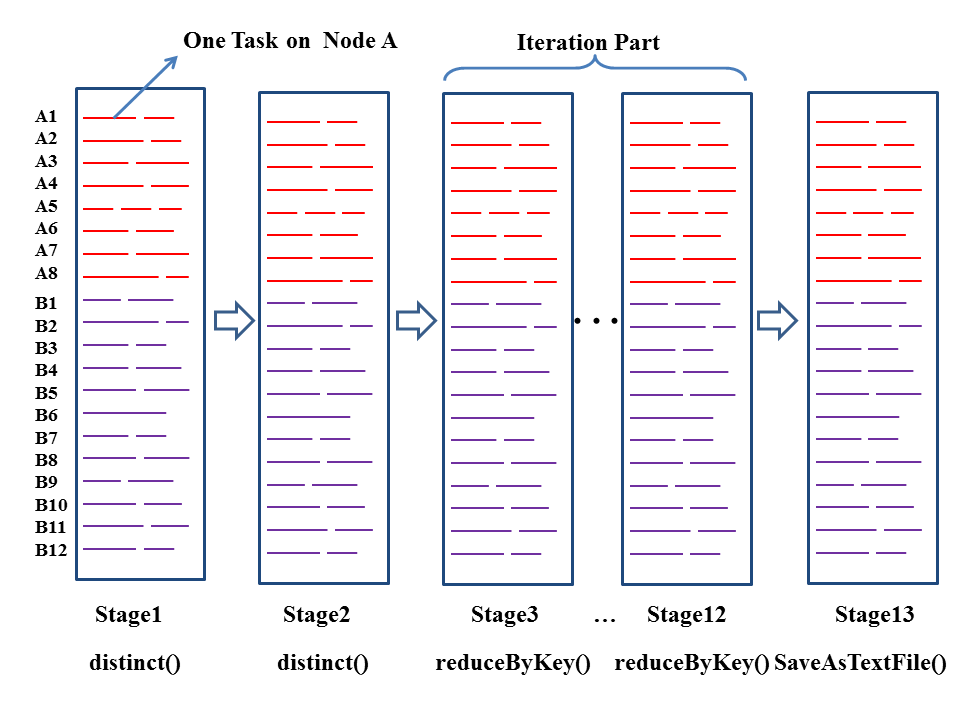
\includegraphics[width=3.0in]{flow.png}
\caption{Prediction Accuracy for WordCount}
\label{flow}
\end{figure}
}
\begin{figure}[!t]
\centering
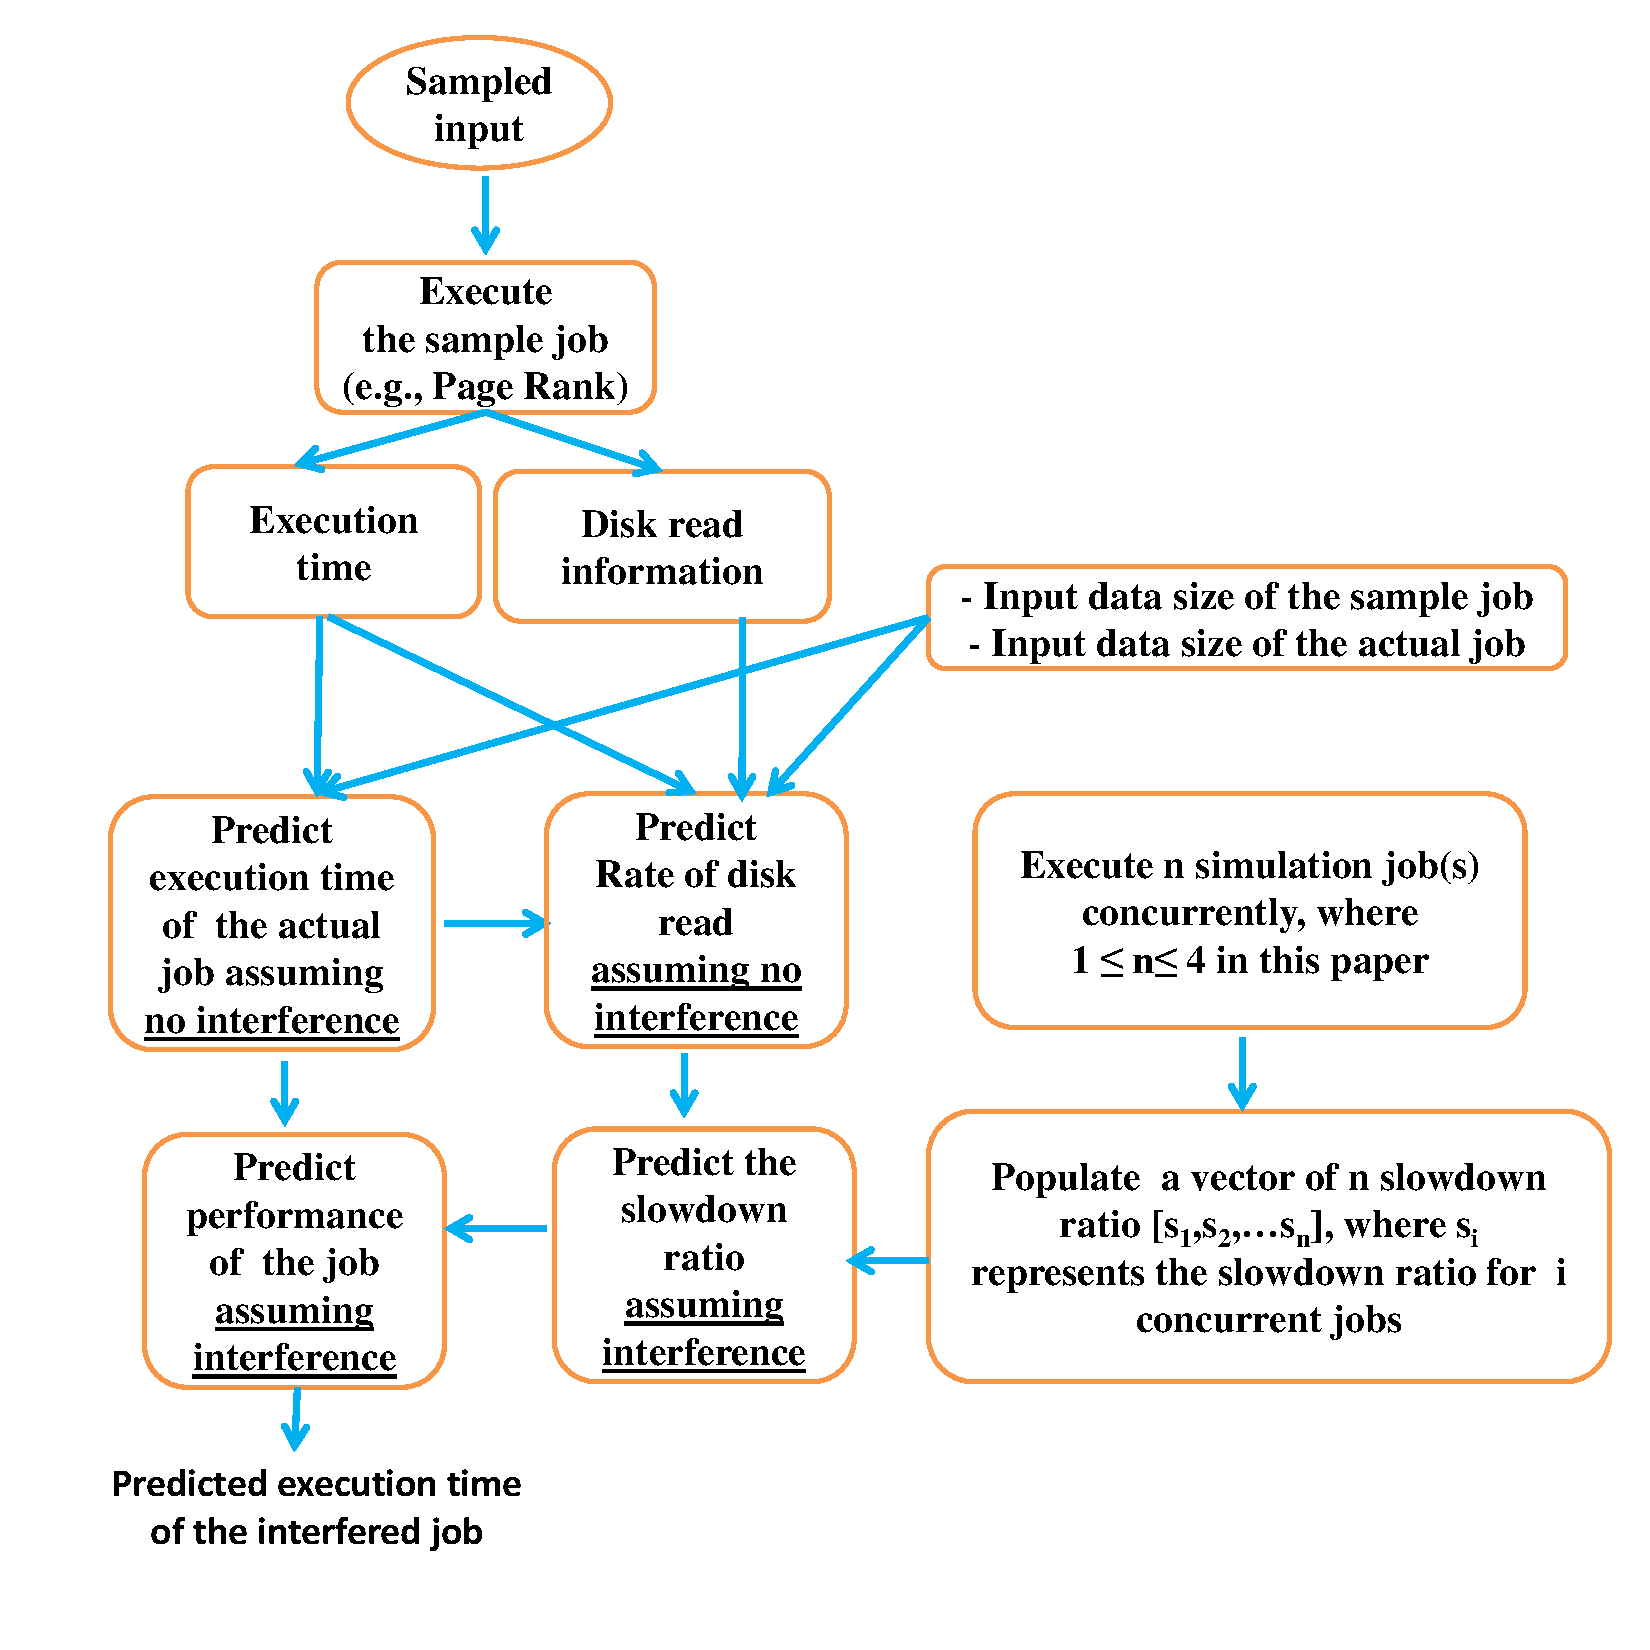
\includegraphics[width=3.3in]{flow1.pdf}
\caption{Performance Prediction for Interfered Jobs}
\label{flow}
\end{figure}

\noindent
Given the above multistage execution model, the main idea behind our work is as follows (Figure~\ref{flow}). First, for a given Apache Spark job, we predict the execution time for each stage leveraging the performance model developed based on the performance of the actual job with smaller input data set. Note that this model is presented in our prior work~\cite{wangperformance}, and assumes that there are no interference in the system from other jobs. Next, we estimate the slowdown ratio for a given number of jobs running concurrently by executing our simulation job, which is implemented by us (more details in Section~\ref{evaluation}) and is different than any of the four jobs that we used for evaluation. However, as the slowdown ratio due to interference among simulated jobs can be different compared to the actual jobs, for a given job, we adjust the expected slowdown ratio by taking into account the actual job parameters such as input data size and disk I/O characteristics. Once we estimate the expected slowdown ratio, we estimate the execution time considering the interference. For completeness, we first briefly present the model that is used to predict execution time assuming no interference from our earlier work~\cite{wangperformance}, and then present the model for predicting the slowdown ratio due to interference that allows us to predict the execution time in the presence of interference among multiple jobs. 


\subsection{Model for Estimating Execution Time}
\label{oldmodel}
As an Apache Spark job is executed in multiple stages where each stage contains multiple tasks, we use the following notation to represent an Apache Spark job.
\begin{IEEEeqnarray}{rCl}
\label{jobperform}
Job &{} ={}& \{Stage_i \mid 0 \leq i \leq M \} \\
Stage_i &{} ={}& \{Task_{i,j} \mid 0 \leq j \leq N \} 
\end{IEEEeqnarray}

\noindent
Here $M$ is the number of stages in a job and $N$ is the number of tasks in a stage. 

\noindent
Next, as different stages within a job are executed sequentially, we represent the execution time of a job as the sum of the execution time of each stage plus the job startup time and the job cleanup time as follows.
\begin{IEEEeqnarray}{rCl}
\label{jobtime}
\hspace{-0.4cm}
JobTime = Startup + \sum_{s=1}^{M}StageTime_{s} + Cleanup
\end{IEEEeqnarray}
Next, within each stage, as one CPU core executes one task at a time, in a cluster with $H$ worker nodes, the number of tasks $P$ that can run in parallel is calculated as follows.

\begin{IEEEeqnarray}{rCl}
\label{paralltask}
P=\sum_{h=1}^H CoreNum_{h}
\end{IEEEeqnarray}

\noindent
Here $CoreNum_{h}$ is the number of CPU cores of working node $h$ and $H$ is the number of working nodes in the cluster. Hence, within an execution stage, tasks in each stage are executed in batches where each batch consists of $P$ tasks running in parallel. However, due to the differences in computing capabilities among different worker nodes in a cluster and inherent uncertainty in program execution, the execution time of different tasks may vary significantly. Therefore, the time spent in a particular stage can be calculated as the maximum of the sum of all the sequential tasks' time within a stage plus the stage startup time and the stage cleanup time as follows.

\begin{IEEEeqnarray}{rCl}
\label{stagetime}
StageTime&{} ={}& Startup + \max_{c=1}^{P} \sum_{i=1}^{K_c} TaskTime_{c,i} \nonumber \\
&&+Cleanup
\end{IEEEeqnarray}

\noindent
Here $P$ is the number of total CPU cores, and $K_c$ is the number of sequential tasks executed on CPU core $c$.

\noindent
Finally, as different tasks in a stage follow the same execution pattern, the execution time of a task can be computed as follows.

\begin{IEEEeqnarray}{rCl}
\label{tasktime}
TaskTime&{} ={}& DeserializationTime + RunTime \nonumber \\
&&+ SerializationTime
\end{IEEEeqnarray}

\noindent
Here $DeserializationTime$ is the time taken to deserialize the input data, $SerializationTime$ is the time taken to serialize the result, and $RunTime$ is the actual time spent performing operations on data such as data mapping, filtering, calculation, and analyses. 
Based on the above model, to predict job performance, the presented framework first executes the program on a cluster using limited amount of sample input data and collects performance metrics such as run time during the simulated run. 

\noindent
Next, to predict the execution time of the actual run based on the extracted performance metric from simulated run, we first calculate the number of tasks $N$ where $ N = InputSize / BlockSize $, $InputSize$ is the size of the input data, and $Blocksize$ is the size of one data block in HDFS. 
The tasks within a stage are scheduled to run batch by batch, and the number of tasks $P$ in each batch is computed as shown in equation (\ref{paralltask}). In one batch of tasks, while the tasks may start simultaneously, they may not finish at the same time due to various factors such as data skew problem, and differences in computing capability of different worker nodes. Hence, using sampled data, we calculate the average execution time for a task for a given stage for a worker node $h$ as follows. 
\begin{IEEEeqnarray}{rCl}
\label{taskest}
TaskRunTime_{h,i} &{} ={}& DeserializeTime_{h,i} \nonumber \\
&&+ RunTime_{h,i} \nonumber \\
&&+ SerializationTime_{h,i} \\
\label{avgtask}
AvgTaskTime_h &{} ={}& \frac{1}{n_h}\sum_{i=1}^{n_h} TaskRunTime_{h,i}
\end{IEEEeqnarray}
Here $n_h$ is the number of tasks running in host $h$ in a particular stage of the sample job. 
Moreover, during our experiment, we observed that the average execution time of the first batch is significantly different compared to the subsequent batches within the same stage, which we capture as follows. 
\begin{IEEEeqnarray}{rCl}
\label{ratio}
Ratio_h=\frac{\frac{1}{n_h-P_h} \sum_{i= P_h + 1}^{n_h}TaskTime_{h,i}}{\frac{1}{P_h} \sum_{j=1}^{P_h} TaskTime_{h,j}}
\end{IEEEeqnarray}
Here $n_h$ is the number of tasks running in host $h$, and $P_h$ is the number of tasks in the first batch. As tasks execute on different hosts in parallel, to predict the execution time for a particular stage during actual execution, stage $Startup$ time and $Cleanup$ time are viewed as constants which are extracted from simulation logs, and stage execution time is estimated as follows.
 
\begin{IEEEeqnarray}{rCl}
\label{stageest}
EstStageTime&{} ={}&Startup + \max_{c=1}^{P} \sum_{i=1}^{K_c} AvgTaskTime_{c,i} \nonumber \\
&& +  Cleanup \\ 
\nonumber \\
\label{stagetask}
EstTaskTime_{c,i}&{} ={}&\left\{\begin{IEEEeqnarraybox}[\relax][c]{l's}
AvgTaskTime_c,& $i = 1$\\
AvgLaterTaskTime_c,& $i > 1$%
\end{IEEEeqnarraybox}\right.
\end{IEEEeqnarray}



\noindent
Here $P$ is the number of total CPU cores calculated in equation (\ref{paralltask}) and $K_c$ is the number of sequential tasks running on CPU core $c$. $AvgTaskTime_c$ is the average time of the tasks of the first batch running on CPU core $c$ for the corresponding host, which is calculated in equation (\ref{avgtask}). $AvgLaterTaskTime_c$ is the average time of the tasks of the following batches, which is calculated as $Ratio_h \times AvgTaskTime_h$.

\noindent
While we can apply the prediction model presented in this section to estimate the execution time for a single job assuming no interference~\cite{wangperformance}, we still need a way to predict the slowdown ratio when interfered with other jobs, which we address as follows.


\subsection{Modeling Interference}
As different stages of a job is expected to have different characteristics in terms of resource utilization (e.g., CPU, I/O, memory), different stages of multiple jobs running concurrently on a system is expected to result in different interference patterns, affecting the execution time differently. Based on this observation, we model the slowdown ratio due to interference among multiple jobs for each stage separately. Towards that, in our model, each stage is represented as a vector consisting of execution time, CPU usage, disk I/O rate, and network I/O rate as follows.
\begin{equation}
\label{res}
Res_i = (RunTime_i, CPU_i, DiskIO_i, NetIO_i)
\end{equation}
Here $1 \leq i \leq M$, and $M$ is the number of stages in a job. Memory was not one of the bottleneck resources in our case. As such, we only considered Disk I/O and did not consider memory utilization in our model, which can be incorporated if needed for certain platforms/scenarios. 





\par \noindent 
Next, the slowdown resulting from interference with other applications for a particular stage is represented as follows.
\begin{equation}
\label{slowdownratio}
SlowdownRatio(Stage_{i,k})
= f(Res_{i,k},Res_{Other jobs})
\end{equation}
\nop{
\begin{equation}
\label{setS}
SetS = \{Stage_{k,i} \mid 1 \leq k \leq J \ , 1 \leq i \leq M \}
\end{equation}
}
\noindent
Here $1 \leq k \leq J$, $1 \leq i \leq M$, $J$ is the number of jobs running in parallel, and $M$ is the number of stages in the Apache Spark job. $Res_{Otherjobs}$ represents the resources consumed by other jobs that are running concurrently with $Stage_{i,k}$. 
Simply put, this slowdown ratio is the ratio between execution time with interference over execution time without interference for a particular stage. Hence, once we estimate the value of the slowdown ratio and the expected execution time when there is no interference, we can estimate the execution time if there are interference with other jobs. 


%Please note that, once we collect the resource usage profile by running sample jobs, we need to estimate the execution time of original job. The difference between original job and sample job is the size of input data, which decides the number of tasks in one stage.
\noindent
As the slowdown happens primarily due to contention for bottleneck resources in the system, to better understand the underlying reasons behind the slowdown, we ran a series of experiments and collected job event logs and resource consumption data, and then extracted the resource usage profile for each stage. Job event log is generated by Apache Spark platform, and resource consumption data is collected using system monitoring tool dstat \cite{dstat}. Apache Spark log records the time line of different stages of a running job, which was used to determine the submission and completion time of different stages of a job. The resource usage for different stages of a job is represented as below: 
\begin{equation}
\label{cpu}
CPU_i 
= (CPUusr_i, CPUsys_i, CPUidle_i, CPUwait_i) 
\end{equation}
\begin{equation}
\label{diskio}
DiskIO_i = (RateofDiskRead_i, RateofDiskWrite_i)
\end{equation}
\begin{equation}
\label{netio}
NetIO_i = (RateofNetReceive_i, RateofNetSend_i)
\end{equation}
Here $1 \leq i \leq M$, and $M$ is the number of stages in a Apache Spark job.
\noindent 
As an Apache Spark job uses in-memory data processing to reduce execution time, in the first stage of a job, it reads the input data to memory, and then analyzes the in-memory data in the subsequent stages. Due to this characteristic, in the first stage, frequent I/O is expected, leading to longer I/O wait. Based on this observation, as bulk of the disk I/O happens in the first stage, in our model, we calculate the slowdown ratio for the first stage only, and assume that the slowdown ratio in cases where the first stage interferes with the following stages from another job is 1.0 (i.e., the slowdown due to interference is expected to be minimal). Note that, while this assumption is not accurate for certain jobs and stages, the error introduced due to this assumption in prediction accuracy is not significant in our case. 

\nop{
In our cluster, the Maximum network transaction speed is 118MB/s tested by using iperf command, and the maximum disk I/O is 266MB/s tested by using dd command. We find that the network I/O or disk I/O speed can not reach the maximum value when we run Apache Spark job in the cluster, but the cpu usage often achieves high value. From this observation, we infer that the bottleneck of Apache Spark job is often in CPU usage, which determines the execution time of the job stage. CPU usage is calculated as the sum of the user and system CPU usage. And high level of CPU usage means the high processing speed in this stage, which will result in less execution time.
}


\noindent 
As most of the time spent in the first stage is due to reading data from disk to memory, we represent the relationship between the amount of data read in the first stage (e.g., size of input data), the rate of disk read, and the execution time of the first stage as follows: 
\begin{equation}
\label{diskread}
RunTime_{Stage 1}=c \times \frac{Input Data Size}{Rate of DiskRead_{Stage 1}} \end{equation}
\noindent 
Now, if we assume that we execute the same job twice, once with the reduced input data set (i.e., sample job) and once with the complete input data set (i.e., complete job), from equation~\ref{diskread}, we can have the following. The word {\textit{Int.}} refers to {\textit{Interference}} in the following equations. 


\begin{eqnarray}
\label{sampleFull}
\begin{gathered}
\frac{InputDataSize_{Sample job}}{InputDataSize_{Complete job}} = \\
\frac{Rate of Disk Read_{Sample job, Stage 1}}{RateofDiskRead_{Complete job, Stage 1}} \times \\
\frac{RunTime_{Sample Job, Stage 1}}{RunTime_{Complete job without Int., Stage 1}}
\end{gathered}
\end{eqnarray}


Based on equation~\ref{sampleFull}, we can have the following equation for predicting the rate of disk read for a complete job. 


\begin{eqnarray}
\label{fullDiskIORead}
\begin{gathered}
Predicted Rate of Disk Read_{Complete Job without Int., Stage1}  = \\
Rate of Disk Read_{Sample Job, Stage 1} \times \\
\frac{RunTime_{Sample Job, Stage 1}}{RunTime_{Complete Job without Int., Stage 1}} \\
\times \frac{Input Size_{Complete Job}}{Input Size_{Sample Job}}
\end{gathered}
\end{eqnarray}

\noindent
In the above equation, we can estimate the value of $RunTime_{Complete Job without Int., Stage 1}$ using the model described in Section~\ref{oldmodel}~\cite{wangperformance}. Once we predict the rate of disk read for a complete job with no interference, next, we need to model the relation between the rate of disk read and the slowdown ratio when there is interference. For that, first, we run a simulation program (written by us as described in Section~\ref{evaluation}) to collect the runtime information with and without interference and calculate the parameter $\beta_{n}$ as follows.
\begin{equation}
\label{beta}
\begin{gathered}
\beta_{n} = \frac{1}{Rate of Disk Read_{Simulation Run without Int., Stage 1}} \times \\
(\frac{RunTime_{Simulation Run with Int. for n jobs, Stage 1}}{RunTime_{Simulation Run without Int., Stage 1}} - \\
\floor*{\frac{RunTime_{Simulation Run with Int. for n jobs, Stage 1}}{RunTime_{Simulation run without Int., Stage 1}}})
\end{gathered}
\end{equation}
\noindent
In this paper, we assume that there can be at most 4 concurrent jobs in a system, and varied $n$ between 2 to 4 to calculate $\beta_{2}$, $\beta_{3}$, and $\beta_{4}$. Running the simulation job and calculating $\beta_{n}$ take only few minutes and need to be done only once for a given environment. Next, we use $\beta_{n}$ to estimate the slowdown ratio when there are $n$ concurrent jobs in the system as follows.

\begin{equation}
\label{slowdisk}
\begin{gathered}
SlowdownRatio(Stage_{(1,k)})=\\
\frac{RunTime_{Complete Job with Int., Stage 1}}{RunTime_{Complete Job without Int., Stage 1}} = \beta_{n} \\
\times PredictedRateofDiskRead_{Complete Job without Int., Stage 1} \\ + \floor*{\frac{Run Time_{Simulation run with Int., Stage 1}}{Run Time_{Simulation Run without Int., Stage 1}}}
\end{gathered}
\end{equation}



\subsection{The Cascading Effect}
Given the above formulation, if we assume that all the jobs are of same type and start at the same time, modeling interference is straightforward as they all have the same execution behavior in each stage. However, for interference among different types of jobs possibly starting at different times, this is a bit more complicated due to the possible cascading effect. For example, the slowdown of stage 1 of job $A$ may push this stage to interfere with stage 2 of job $B$. Hence, a dynamic interference estimation algorithm is designed to solve this problem. The main idea behind the algorithm is as follows. First, the algorithm uses the execution time line of each job as input, and calculates the slowdown ratio for each stage of different jobs within the same time slot, and generates the execution time line of each job under interference condition. Based on that, the algorithm identifies the job that will finish its first stage the earliest, removes that job from the list, and recalculates the effect of interference for the remaining jobs for the remainder of the execution time. The algorithm applies this repeatedly until the list becomes empty. This dynamic interference estimation algorithm is described in Algorithm~\ref{algo} (Appendix).





\subsection{Interference Aware Job Scheduling}
\label{scheduler}

Finally, as concurrent Apache Spark jobs often heavily interfere, especially at the first stage, to minimize interference and job execution time, we design and implement a scheduler that automatically schedules and executes submitted Spark jobs leveraging the performance prediction framework presented earlier. Specifically, when a new job arrives in the system, if there is no existing job in the system, the scheduler locates available servers that can execute the job and starts the job immediately. However, if there are existing jobs running in the system with possibly more jobs waiting in the queue, the scheduler calculates the waiting time (if any) of the new job and readjusts the waiting time of the jobs that are already in the queue (if needed) to determine the best scheduling plan and updates the scheduling file accordingly (Note that jobs are not executed on first-come-first serve basis in our system). 

\noindent
The process of calculating the waiting time for a job in multiple steps is illustrated in Figure \ref{scheexample}. Here we assume that the first job $J_1$ is submitted at time point $T_1$, and is started immediately as there is no other job in the system. The second job $J_2$ is submitted at time $T_2$. At that time, the scheduling algorithm calculates the amount of time already executed by $J_1$ (i.e., $T_2-T_1$) to decide whether $J_2$ can be started immediately or needs to wait to avoid interference. If $J_2$ needs to wait, the algorithm calculates the tentative wait time for $J_2$ based on the interference model, which is $\Delta T$, and updates the scheduling file by writing the waiting period $\Delta T$ for $J_2$.

\noindent
Now, let us assume that, at time point $T_3$, the third job $J_3$ arrives in the system. At that point, the algorithm first calculates the execution time (which is different than the wall clock time) of the two jobs already running in the system. As $J_1$ executed alone before $S_1$ and executed concurrently with $J_2$ between $S_1$ and $T_3$, we calculate the execution time of $J_1$ since the last job submission time (i.e., $T_2$) as $ExeTime_{J1} = (S_1-T_2)+(T_3-S_1) \times Ratio_{J_1}$, and the execution time for $J_2$ as $ExeTime_2 = (T_3-S_1) \times Ratio_{J_2}$, where $Ratio_{J_1}$ and $Ratio_{J_2}$ are the slow down ratio of $J_1$ and $J_2$ respectively when interfered with one job. Note that the slowdown ratios are different for different jobs due to differences in job characteristics. Also, as the job profiles in the scheduling file are updated every time a new job is submitted, we only need to estimate the execution time for each running job since the last job submission time. 

\noindent
After calculating the execution times for these two jobs (which tell us what stage each job is at currently), we update the job profiles for $J_1$ and $J_2$, and then decide whether $J_3$ can start immediately or not, based on the possibility of interference with the currently running jobs. 

\noindent
While calculating the execution time, we have to consider the possibility that each job may interfere with different jobs at different points in time during the execution. To handle this possibility, the algorithm saves the start and end time point of the first stage for each job (as the significant interference happens in the first stage of a job), and sorts the list based on start time points, and determines which set of jobs interfere at a particular point in time, and calculates the execution time incrementally. 

\begin{figure}[!t]
\centering
\captionsetup{justification=centering}
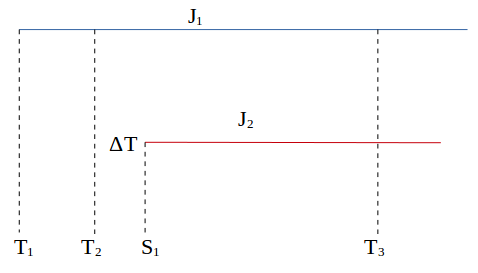
\includegraphics[width=3in]{ScheExample.png}
\caption{A Scheduling Example}
\label{scheexample}
\end{figure}




\noindent




\noindent
The algorithm to determine the waiting time for a job is shown in Algorithm~\ref{algoschedule} (Appendix) which has two main parts. The first part of the algorithm consists of the function depicted in Algorithm~\ref{algoexe} (Appendix) that calculates the execution time of the previously submitted jobs and updates the job schedule file (Algorithm~\ref{algoupdate} (Appendix)). The second part consists of Algorithm~\ref{algofind}(Appendix) that searches the combination of waiting times and job schedules that will minimize the total execution time. 











